\section{Implémentation}
\subsection{BruteForce}
L'implémentation de l’algorithme d’énumération de chemins et circuits par force brute utilise la librairie de gestions de graphes mise à disposition des étudiants sur le site discmath. Toute interaction de l’application se fait en ligne de commande via les arguments de l’exécutable. L’utilisateur peut ainsi choisir le type de parcourt ouvert ou fermé ainsi que la taille de l’échiquier en X et en Y.  Cela permet la création de scripts pour automatiser l’exécution qui peut prendre un temps considérable pour des tailles importantes d’échiquier.
Lors de l’initialisation, un graphe représentant les cases accessibles à partir de chaque case est crée. Ensuite une fonction récursive parcourt ce graphe en fonction de la liste d’adjacence de chaque nœud et des cases déjà visitées.

Cet algorithme de parcourt récursif est appelé pour chaque case de départ possible. Cela permet de créer un tableau montrant le nombre de chemins existants en fonction de la position de départ. L’utilisateur peut voir l’évolution du calcul en temps réel dans le terminal.
\begin{table}[H]
\centering
\caption{Tableau crée pour une recherche de chemins sur un échiquier de taille 5*5}
\label{my-label}
\begin{tabular}{lllll}
304 & 0  & 56 & 0  & 304 \\
0   & 56 & 0  & 56 & 0   \\
56  & 0  & 64 & 0  & 56  \\
0   & 56 & 0  & 56 & 0   \\
304 & 0  & 56 & 0  & 304
\end{tabular}
\end{table}
\subsection{Génération de chemins et circuits hamiltoniens}
Pour la partie du code concernant la génération de circuits et chemins sur des échiquiers de taille variable, nous avons implémenté trois fonctions, pour les trois algorithmes sélectionnés :
\begin{itemize}
\item Heuristique de Warnsdorff pour trouver un chemin ou un circuit sur un échiquier carré ou rectangulaire avec départage aléatoire.
\item Algorithme de Squirrel pour trouver à coup sur un chemin sur un échiquier carré.
\item Algorithme de Shun-Shii pour le cas d'un échiquier de trois lignes et m colonnes. Permettant de trouver un chemin hamiltonien.
\end{itemize}
\subsubsection{Génération de parcours et chemins}
Dans ces fonctions, nous enregistrons l'ordre de parcours des cases dans un vecteur A. Le premier élément de ce vecteur représente la case en haut à gauche. Le dernier élément représente la case en bas à droite. Comme si les rangées de l'échiquier avaient été mises bout à bout. Les éléments contiennent comme valeur l'ordre de passage du cavalier sur la case correspondante. Allant donc de 0 à n*m-1. Un vecteur B contient le poids des cases, comme sur la figure ~\ref{cavalier_graphe}. Il est à noter que tous nos algorithmes commencent dans la case en haut à droite de l'échiquier. Théoriquement, l'algorithme avec départage aléatoire pourrait commencer sur n'importe quelle case. Mais par facilité, nous avons décidé arbitrairement de celle-ci.

Afin de minimiser les temps de calcul, le lancement de la fonction de parcourt se fait en multithreading via OpenMP. Ainsi un thread travaille sur chaque case initiale possible.

Au début, nous avions décidé d'utiliser l'interface de génération de graphes vue au cours, en la modifiant légèrement. Cependant, le résultat obtenu avec l'algorithme de Warnsdorff était trop compliqué et trop lent. Nous avons donc décidé de nous inspirer de l'algorithme de Squirrel, basé sur les matrices décrite au paragraphe précédent.
Le fonctionnement des algorithme a été décrit au chapitre précédent. 

\subsubsection{Test de la validité des parcours et chemins}
Pour vérifier la justesse des parcours et chemins générés, nous avons écrit deux fonctions de test. L'une pour les parcours et l'autre pour les chemins. Leur fonctionnement est pratiquement identique. L'algorithme commence à la case "0". On regarde ensuite si la case "1" est accessible en un mouvement de cavalier. Si oui, on s'y déplace,... Si toutes les cases ont pu être visitées, le chemin est valide. Pour le test de circuits, on vérifie en plus si la case "0" est accessible depuis la case "n*n-1".

\subsubsection{Affichage du résultat}
En plus de la génération, nous proposons d'enregistrer le résultat obtenu dans un fichier texte. La figure ~\ref{ExempleImpression} montre plusieurs exemples de parcours générés.

\begin{figure}[h]
\begin{center}
   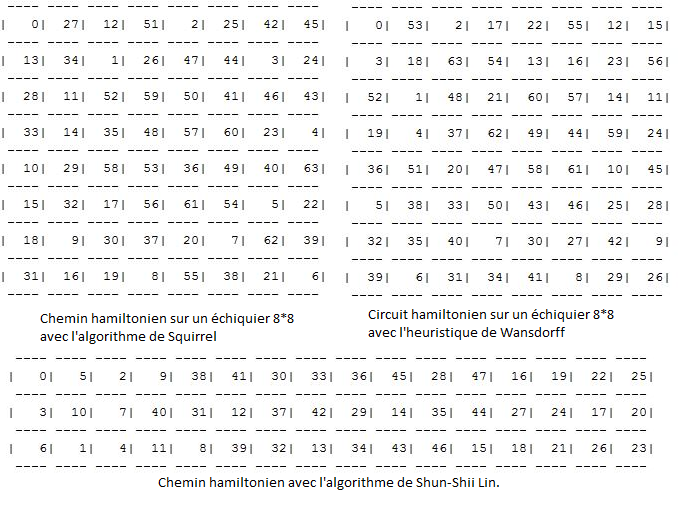
\includegraphics[scale=0.6]{img/exempleimpression.png} 
   \caption{\label{ExempleImpression} Exemple de chemins et circuits générés}
   \end{center}
\end{figure}